\documentclass[14pt,russian]{beamer}

\usepackage[utf8]{inputenc}
\usepackage[T2A]{fontenc}
\usepackage[russian]{babel}

\graphicspath{{presentation/figures/}}

\usecolortheme{dolphin}
\usefonttheme{serif}
\usefont{T2A}{ftm}{m}{sl}

\title{Программное средство для обнаружения радиосигналов с помощью SDR-приемника}
\author{Михолап А.А.}

\institute{Белорусский государственный университет информатики и радиоэлектроники}
\date{Минск, 2015}
\subject{Computer Science}

\begin{document}

\begin{frame}
  \titlepage
\end{frame}


\section{SDR}

\begin{frame}
  \frametitle{Понятие SDR}
  Software-Defined Radio --- это радиосистема, в которой большая часть приемопередающего тракта реализована в виде программного обеспечения.\\
  \vspace{1cm}
  Идея:
  \begin{itemize}
    \item{Минимум железа}
    \item{Максимум софта}
  \end{itemize}
\end{frame}

\begin{frame}
  \frametitle{Software-Defined Radio}
  Преимущества:
  \begin{itemize}
    \item{Изменение характеристик обновлением "<прошивки">: поддержка новых прокотолов связи, криптографических алгоритмов, динамическая подстройка под условия работы и т.д.}
  \end{itemize}
  Недостатки:
  \begin{itemize}
    \item{Нуждается в вычислительном устройстве}
    \item{Менее производителен чем узкоспециализированные системы}
  \end{itemize}
\end{frame}

\begin{frame}
  \frametitle{Software-Defined Radio}
  \begin{figure}
    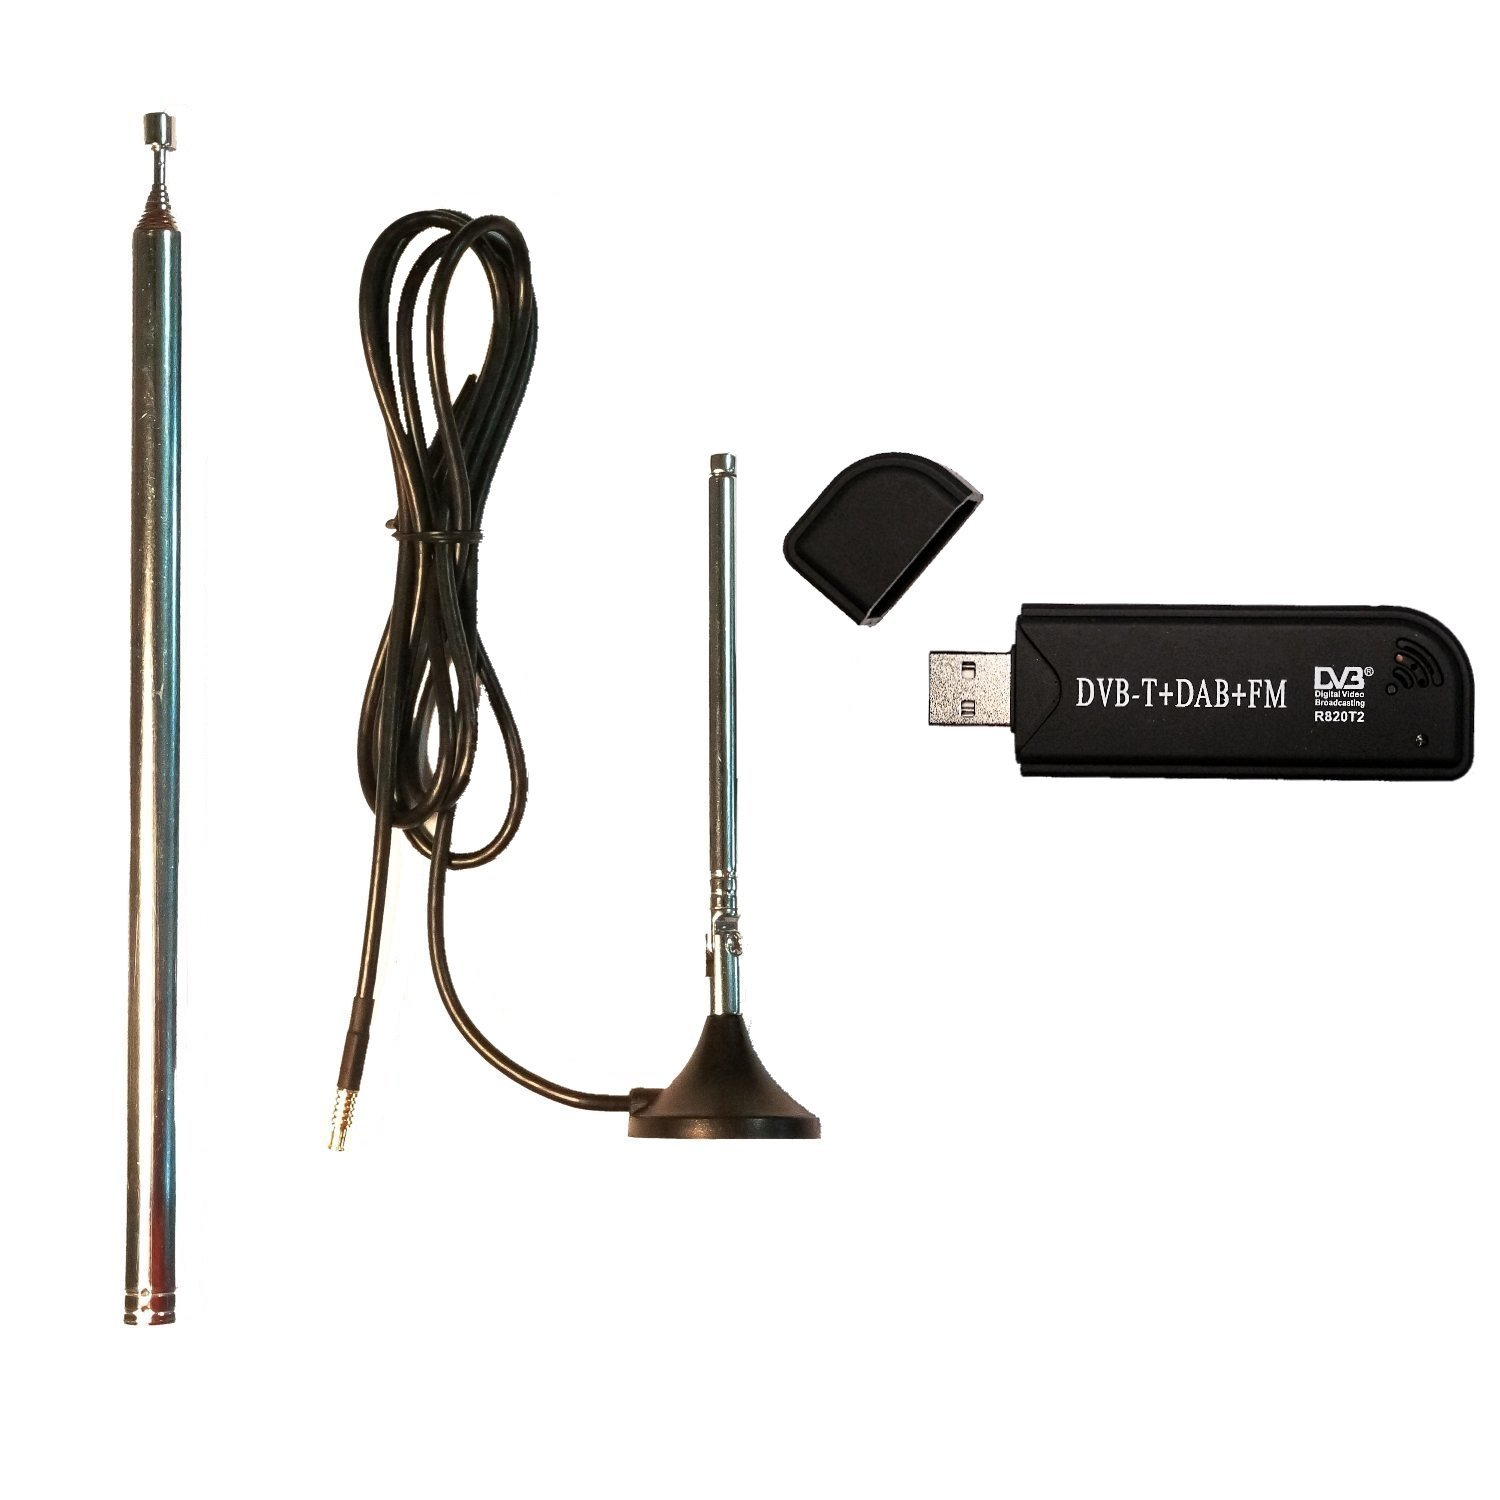
\includegraphics[height=0.8\textheight]{rtl_sdr_set}
  \end{figure}
\end{frame}

\begin{frame}
  \frametitle{Пример: эволюция компьютерных сетей}
  \begin{figure}
    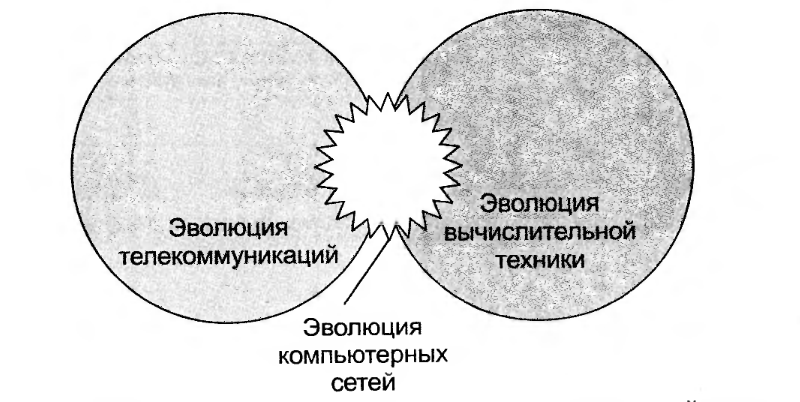
\includegraphics[width=\textwidth]{compnet_evolution}
  \end{figure}
\end{frame}

\begin{frame}
  \frametitle{Эволюция SDR}
  \begin{figure}
    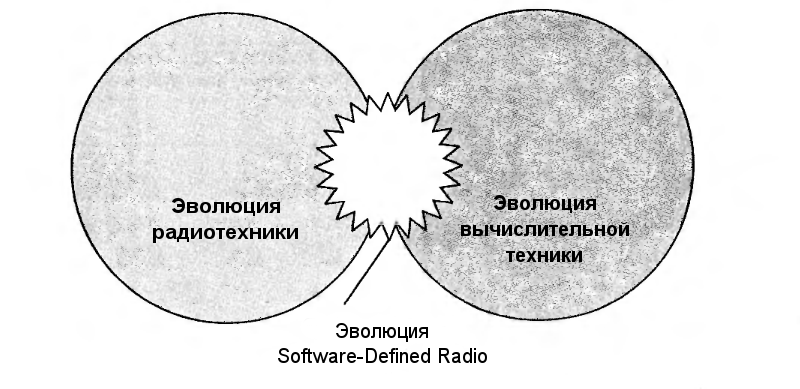
\includegraphics[width=\textwidth]{sdr_evolution}
  \end{figure}
\end{frame}

\begin{frame}
  \frametitle{SDR сегодня}
  \begin{itemize}
    \item{Начало коммерческого производства}
    \item{Использование в военных целях (армия США)}
    \item{Завоевание популярности у радиолюбителей}
  \end{itemize}
\end{frame}


\section{Обнаружение радиосигналов}

\begin{frame}
  \frametitle{Задача}
  \begin{itemize}
    \item{Обнаружение радиосигналов --- фундаментальная задача в своей области}
    \item{Не существует единственно верной формулировки}
    \item{В дипломном проекте решалась проблема выделения частот, содержащих нещумовую активность}
  \end{itemize}
\end{frame}

\begin{frame}
  \frametitle{Трудности}
  \begin{itemize}
    \item{Что считать нешумовой активностью?}
    \item{Никаких априорных сведений о мощности/ширине полосы частот/характере сигнала}
  \end{itemize}
\end{frame}

\begin{frame}
  \frametitle{Идея решения}
  \begin{itemize}
    \item{Ограничиться некоторым подмножеством типов сигналов}
    \item{Для каждого типа разработать алгоритм, учитывающий его специфику}
    \item{Создать систему, агрегирующую результаты их работы}
  \end{itemize}
\end{frame}

\begin{frame}
  \frametitle{Примененные методы}
  \begin{itemize}
    \item{Исследование частотно-временного представления сигнала (спектрограмма)}
    \item{Моделирование временных рядов ($\mathit{ARMA}$)}
    \item{Математическая статистика}
  \end{itemize}
\end{frame}

\begin{frame}
  \frametitle{Спектрограмма сигнала коммерческой FM радиостанции}
  \begin{figure}
    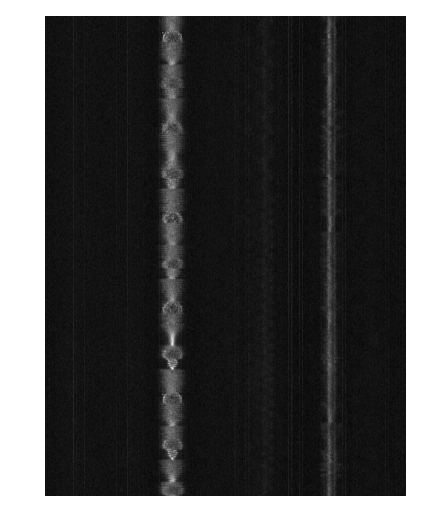
\includegraphics[height=0.7\textheight]{wfm_spectrogram}
  \end{figure}
\end{frame}

\begin{frame}
  \begin{center}
    \Huge{Доклад окончен}
  \end{center}
\end{frame}

\end{document}
